\documentclass[12pt,german]{article}

\usepackage[left=2cm, right=2cm, top=2cm, bottom=3.5cm, landscape=false]{geometry}

\usepackage{graphicx}
\usepackage{float}

\usepackage{tabularx}
\usepackage{booktabs}
\usepackage{dcolumn}

\usepackage{pgfplots}
% \pgfplotsset{compat=1.16}

\usepackage[ngerman]{babel}

\usepackage{amsmath}

\title{\vspace{-1cm}Protokoll Steuerstabskalibrierung}
\author{Fuchs, Gutmann, Kosbab, Kowal, Steindorf, Fälker, Scheffel, Richter}

\begin{document}
    \maketitle
    \tableofcontents

    \section{Kurzbeschreibung des Versuches}
    \begin{itemize}
        \item Die Funktionskontrolle des Reaktors wird gemäß Prüfvorschrift durchgeführt und protokolliert.
        \item Der Reaktor wird durch Wiederholungsstart in Betrieb genommen. Zuerst wird Steuerstab 2 komplett ausgefahren, mit Steuerstab 1 wird der Reaktor dann bei 0,3 W kritisch gemacht.
              Die Steuerstabsstellung ist hierbei (S1: 3645, S2: 0, S3: 4000).
        \item S2 wird um 800 Einheiten eingefahren, eine Minute wird gewartet und anschließend die Verdopplungszeit per Hand gemessen.
        \item Nach Beenden der Messung wird S3 eingefahren um den Reaktor wieder bei 0,3 W kritisch zu machen.
        \item Dieser Vorgang wird 5 mal wiederholt bis S2 komplett ausgefahren ist.
    \end{itemize}

    \newpage

    \section{Messwerttabelle mit Angabe der Messfehler}
    \begin{table}[H]
        \begin{tabularx}{\textwidth}{X|X|X|X|X|X|X|X|X}
            \toprule
            & \multicolumn{3}{c|}{\textbf{Stabstellung}} & \multicolumn{4}{c|}{\textbf{Verdopplungszeit}} & \textbf{Periode} \\
            \cmidrule{2-4}\cmidrule{5-8}
            % \midrule
            P & $S1$ & $S2$ & $S3$ & $T_{WB\: 1}$ & $T_{WB\: 2}$ & $T_{LB}$ & $\overline{T_{2}}$ & $T_s$ \\
            \midrule
            $0.32\, W$ & $3465$ & $   0$ & $4000$ & $  \infty  $ & $  \infty  $ & $  \infty  $ & $  \infty  $ & $  \infty  $ \\
            $0.92\, W$ & $3465$ & $ 827$ & $4000$ & $198.87\, s$ & $198.80\, s$ & $193.03\, s$ & $196.90\, s$ & $284.07\, s$ \\
            $0.32\, W$ & $3465$ & $ 827$ & $3440$ & $  \infty  $ & $  \infty  $ & $  \infty  $ & $  \infty  $ & $  \infty  $ \\
            $1.42\, W$ & $3465$ & $1604$ & $3440$ & $100.00\, s$ & $101.00\, s$ & $ 97.84\, s$ & $ 99.61\, s$ & $143.71\, s$ \\
            $0.30\, W$ & $3465$ & $1604$ & $2698$ & $  \infty  $ & $  \infty  $ & $  \infty  $ & $  \infty  $ & $  \infty  $ \\
            $1.69\, W$ & $3465$ & $2409$ & $2698$ & $ 71.78\, s$ & $ 72.17\, s$ & $ 70.81\, s$ & $ 71.59\, s$ & $103.28\, s$ \\
            $0.29\, W$ & $3465$ & $2409$ & $1881$ & $  \infty  $ & $  \infty  $ & $  \infty  $ & $  \infty  $ & $  \infty  $ \\
            $1.57\, W$ & $3465$ & $3215$ & $1881$ & $ 76.84\, s$ & $ 75.57\, s$ & $ 73.66\, s$ & $ 75.36\, s$ & $108.72\, s$ \\
            $0.30\, W$ & $3465$ & $3215$ & $1000$ & $  \infty  $ & $  \infty  $ & $  \infty  $ & $  \infty  $ & $  \infty  $ \\
            $1.17\, W$ & $3465$ & $4000$ & $1000$ & $113.59\, s$ & $112.34\, s$ & $107.50\, s$ & $111.14\, s$ & $160.35\, s$ \\
            $1.17\, W$ & $3419$ & $4000$ & $   0$ & $  \infty  $ & $  \infty  $ & $  \infty  $ & $  \infty  $ & $  \infty  $ \\
            \bottomrule
        \end{tabularx}
        \caption{Steuerstabsstellungen und Verdopplungszeiten}
    \end{table}
    \subsection{Messfehler / Potenzielle Fehlerquellen}
    \begin{itemize}
        \item Ungenauigkeiten beim Stoppen der Zeit (Reaktionszeit)
        \item Ungenauigkeiten beim Ablesen der Impulsrate, Leistung und Steuerstabspositionen
        \item Kompromiss beim Warten auf stabile Periode
        \item Differenz zwischen Messkanälen, Abweichung vom Mittelwert
    \end{itemize}
    Die Standartabweichung von den Mittelwerten der Verdopplungszeiten ist im Durchschnitt $2.1s$.

    \section{Rechnerische Auswertung und Diskussion der Fehler}
    \subsection{INHOUR-Gleichung}
    Zur Berechnung der Reaktivität wurde die in der Praktikumsanleitung erläuterte INHOUR-Gleichung 
    sowie die gegeben Werte für $ l^* / \beta $ sowie $ a_i $ bzw. $ \lambda_i $ verwendet:
    \begin{equation*}
        \rho' = \frac{l^* / \beta}{T_S} + \sum^6_{i=1} \frac{a_i}{1 + \lambda_i \cdot T_S}
    \end{equation*}
    Für den AKR gilt $ l^* / \beta = 0.0051 s $.
    \begin{table}[H]
        \centering
            \begin{tabularx}{0.5\textwidth}{X|X|X}
            \toprule
            $ \mathbf{i} $ & $ \mathbf{\lambda_i [s^{-1}]} $ & $ \mathbf{a_i = \beta_i / \beta} $ \\
            \midrule
            $ 1 $ & $ 0.0124 $ & $ 0.033 $ \\
            $ 2 $ & $ 0.0305 $ & $ 0.219 $ \\
            $ 3 $ & $ 0.111 $ & $ 0.196 $ \\
            $ 4 $ & $ 0.301 $ & $ 0.395 $ \\
            $ 5 $ & $ 1.14 $ & $ 0.115 $ \\
            $ 6 $ & $ 3.01 $ & $ 0.042 $ \\
            \bottomrule
        \end{tabularx}
        \caption{Daten der verzögerten Neutronen zur Verwendung in der INHOUR-Gleichung}
    \end{table}
    \subsection{Rechenergebnisse}

    Um die differentielle Reaktivität besser vergleichen und darstellen zu können wird sie zusätzlich im Format $\frac{d\rho'}{dz}*1000$ berechnet.

    \begin{table}[H]
        \begin{tabularx}{\textwidth}{X|X|X|X|X}
            \toprule
            \textbf{S2} & \textbf{Periode} & \textbf{Diff. Reakt.} & \textbf{$\frac{d\rho'}{dz}*1000$} & \textbf{Intgr. Reakt.} \\
            \midrule
            $   827$ & $284.07\, s$ & $0.0410$ & $0.0495$ & $0.0410\, \$$ \\
            $  1604$ & $143.71\, s$ & $0.0739$ & $0.0951$ & $0.1148\, \$$ \\
            $  2409$ & $103.28\, s$ & $0.0964$ & $0.1198$ & $0.2113\, \$$ \\
            $  3215$ & $108.72\, s$ & $0.0926$ & $0.1149$ & $0.3039\, \$$ \\
            $  4000$ & $160.35\, s$ & $0.0674$ & $0.0859$ & $0.3713\, \$$ \\
            \bottomrule
        \end{tabularx}
        \caption{Stellung von Steuerstab 2 mit zugehörigen berechneten Werten}
    \end{table}

    \noindent
    Die Positionen für Steuerstab 3 sind die tatsächlichen Positionen, jedoch in umgekehrter Reihenfolge, da die Steuerstäbe zur Kompensationsmethode eingefahren werden. \\
    Die Positionen für Steuerstab 1 werden aus den Positionen für Steuerstab 2 und 3 gemittelt.

    \begin{table}[H]
        \begin{minipage}[t]{0.475\textwidth}
            \begin{tabularx}{\textwidth}{X|X|X}
                % \toprule
                \multicolumn{3}{c}{\textbf{S3}} \\
                % \cmidrule{2-3}\cmidrule{5-6}
                \midrule
                Position & \textbf{$\frac{d\rho'}{dz}*1000$} & \textbf{$\rho'_{Int}$} \\
                \midrule
                $  1000$ & $0.0410$ & $0.0674\, \$$ \\
                $  1881$ & $0.0838$ & $0.1600\, \$$ \\
                $  2698$ & $0.1180$ & $0.2564\, \$$ \\
                $  3440$ & $0.1248$ & $0.3303\, \$$ \\
                $  4000$ & $0.1204$ & $0.3713\, \$$ \\
                \bottomrule
            \end{tabularx}
        \end{minipage}
        \hfill
        \begin{minipage}[t]{0.475\textwidth}
            \begin{tabularx}{\textwidth}{X|X|X}
                % \toprule
                \multicolumn{3}{c}{\textbf{S1}} \\
                % \cmidrule{2-3}\cmidrule{5-6}
                \midrule
                Position & \textbf{$\frac{d\rho'}{dz}*1000$} & \textbf{$\rho'_{Int}$}\\
                \midrule
                $ 913.5$ & $0.0495$ & $0.0542\, \$$ \\
                $1742.5$ & $0.0951$ & $0.1374\, \$$ \\
                $2553.5$ & $0.1198$ & $0.2339\, \$$ \\
                $3327.5$ & $0.1149$ & $0.3171\, \$$ \\
                $4000.0$ & $0.0859$ & $0.3713\, \$$ \\
                \bottomrule
            \end{tabularx}
        \end{minipage}
        \caption{Stellung von Steuerstab 3 sowie 1 und deren Reaktivität}
    \end{table}

    \section{Grafische Darstellung der Steuerstabkennlinien}
    \subsection{Differentiell}
    \begin{figure}[H]
        \centering
        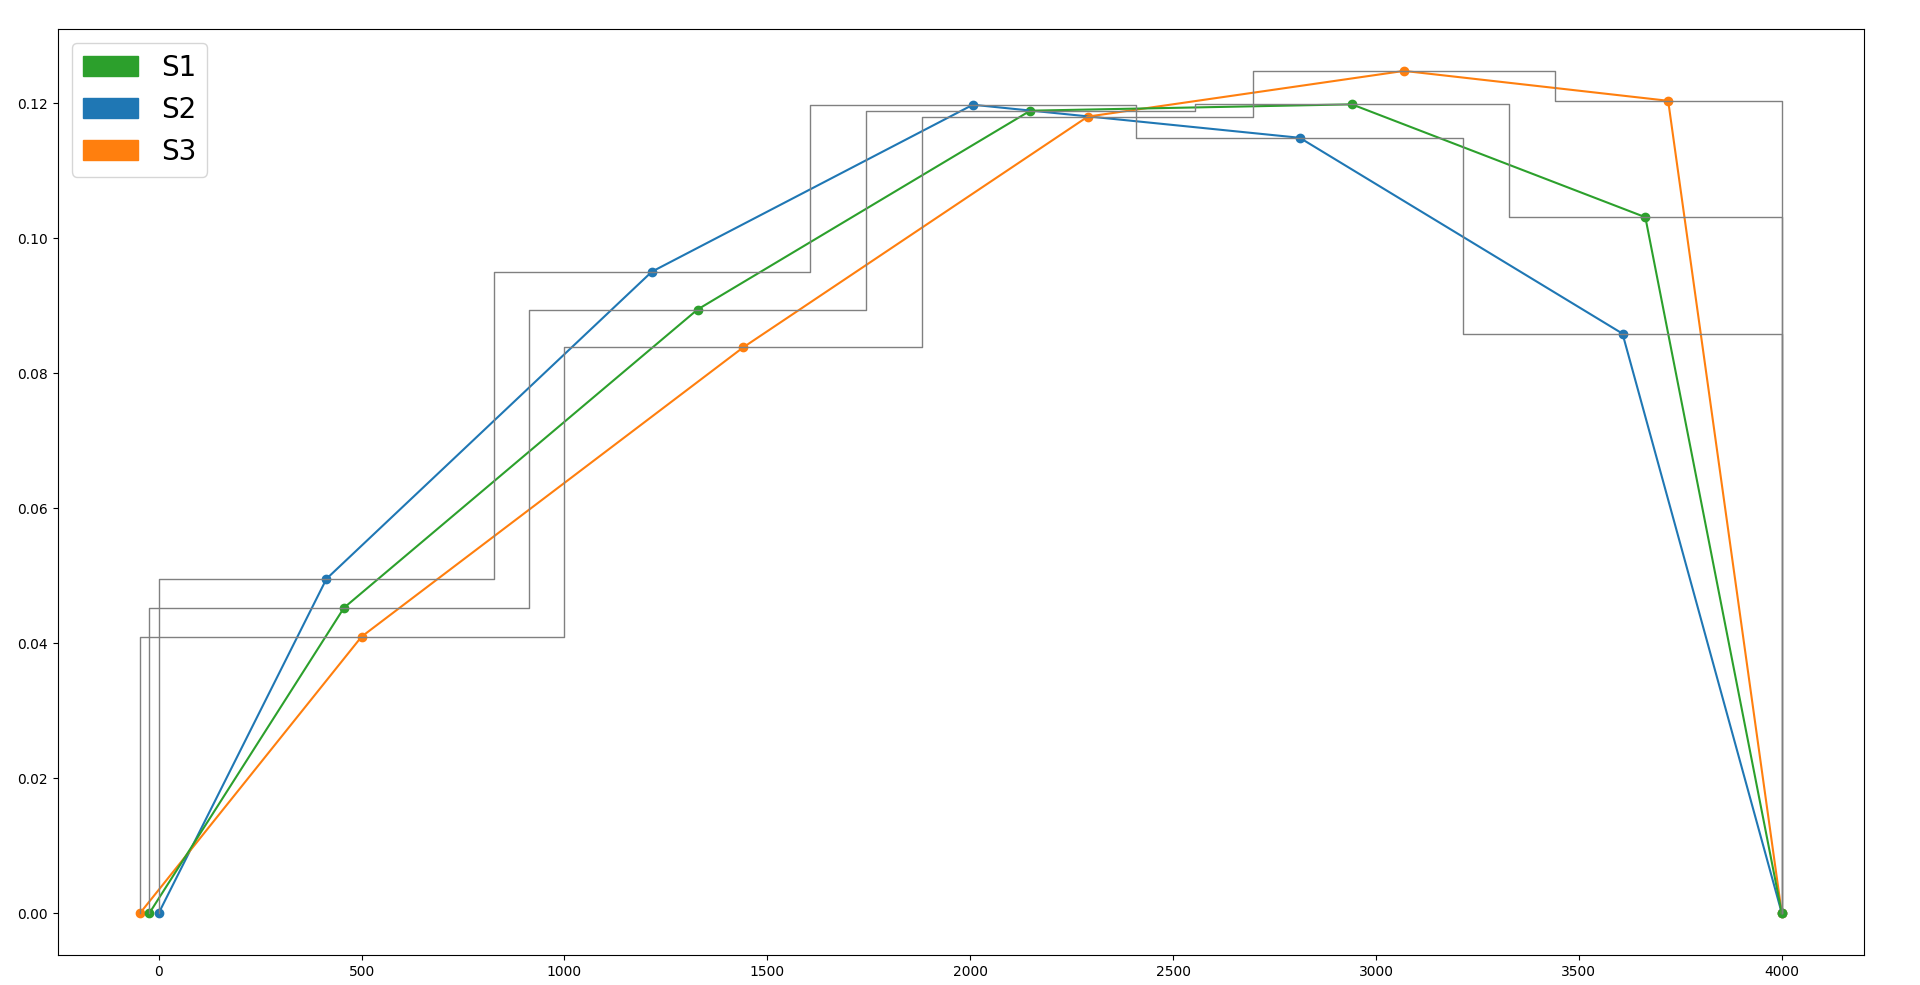
\includegraphics[width=0.9\textwidth]{kennlinien_differential.png}
        \caption{Differentielle Reaktivitätskennlinien}
    \end{figure}
    \subsection{Integral}
    \begin{figure}[H]
        \centering
        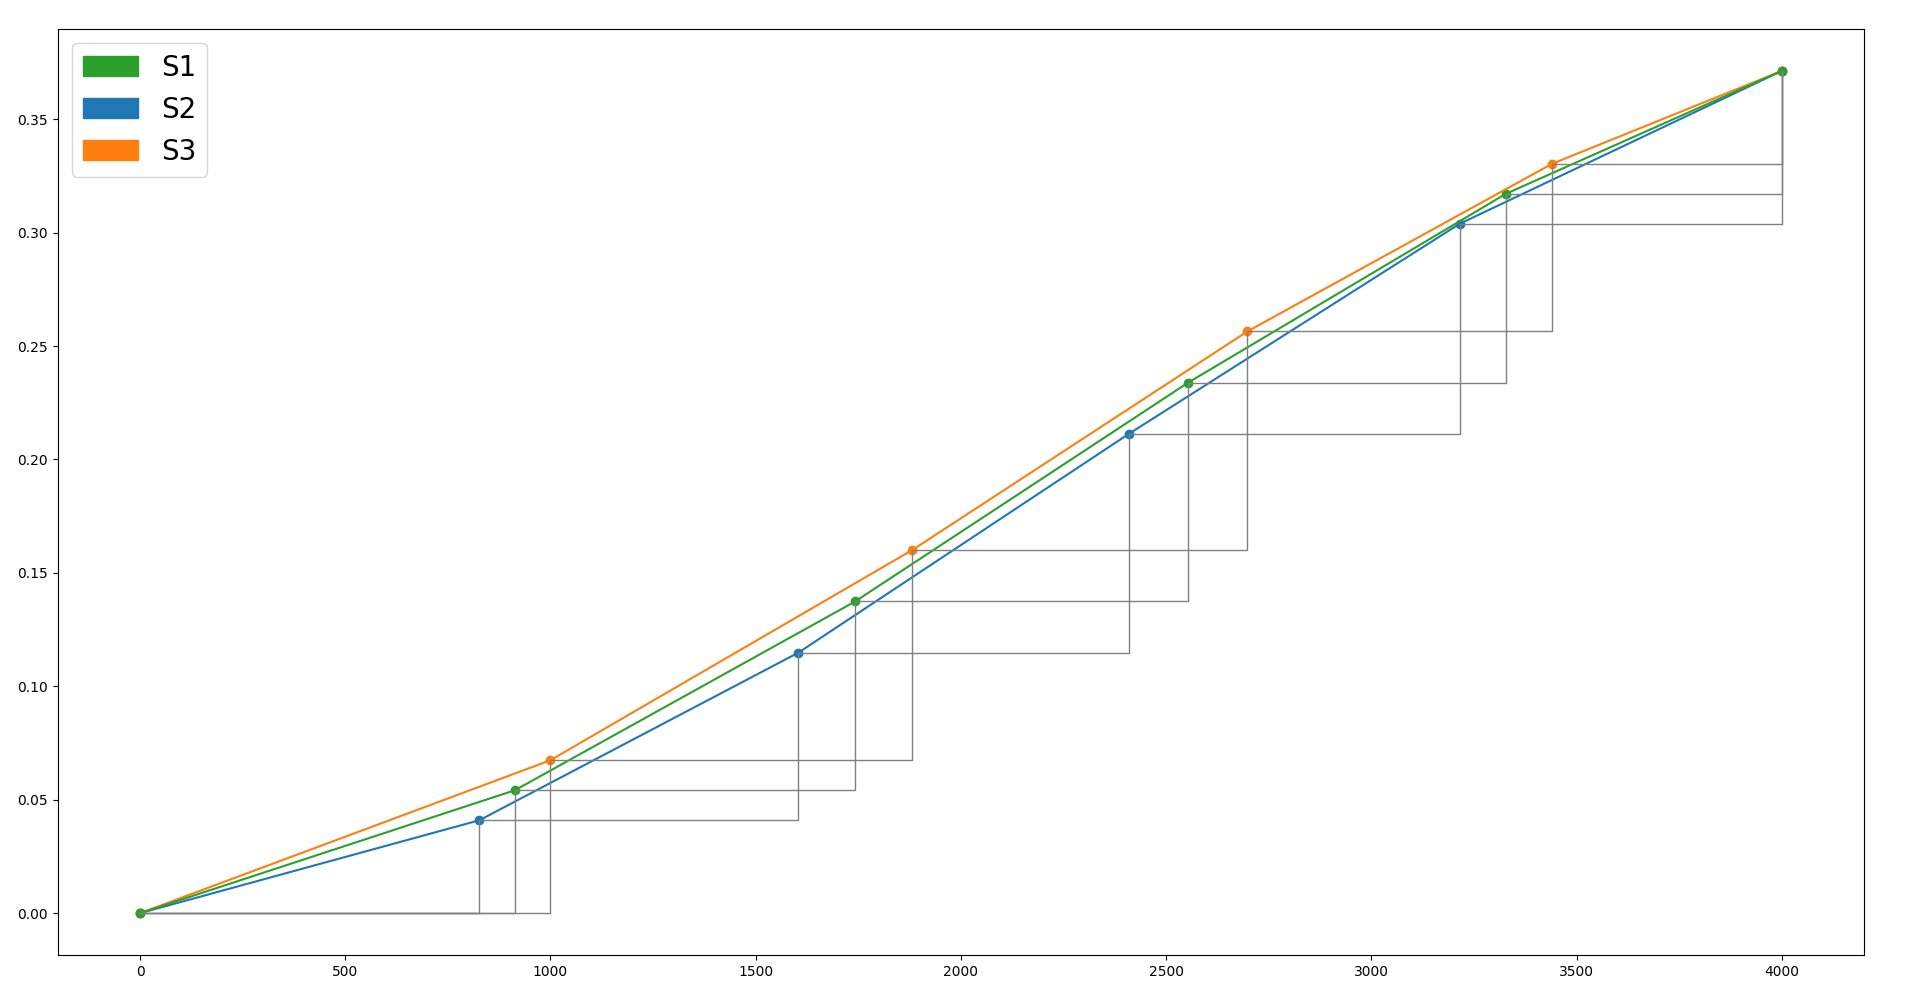
\includegraphics[width=0.9\textwidth]{kennlinien_integral.png}
        \caption{Integrale Reaktivitätskennlinien}
    \end{figure}

    \section{Ableitung der Überschuss- und Abschaltreaktivität}
    \subsection{Gesamtreaktivität}
    Zur Berechnung der Überschuss- bzw. Abschaltreaktivität wird sowohl die Gesamtreaktivität der einzelnen Steuerstäbe, 
    aus auch die des gesamten Reaktors benötigt.
    Die Gesamtreaktivität der Steuerstäbe entspricht der Reaktivitätsdifferenz des jeweiligen Stabes über die gesamte Hubhöhe,
    und ist damit in unserem Fall äquivalent zum Maximalwert der integralen Reaktivität des Stabes.
    \begin{table}[H]
        \centering
        \begin{tabularx}{0.5\textwidth}{X|X}
            \toprule
            \textbf{Steuerstab i} & $\mathbf{\rho'_{i, Gesamt}}$ \\
            \midrule
            $ S1 $ & $0.3712\, \$$ \\
            $ S2 $ & $0.3712\, \$$ \\
            $ S3 $ & $0.3712\, \$$ \\
            \bottomrule
        \end{tabularx}
        \caption{Gesamtreaktivitäten der Steuerstäbe}
    \end{table}
    \noindent Die Gesamtreaktivität berechnet sich anschließend aus der Summe der Gesamtreaktivitäten der einzelnen Steuerstäbe: \\
    \begin{align*}
        \rho'_{Gesamt} &= \sum_{[S1, S2, S3]} \rho'_{i, Gesamt} \\
        &= 0.3712\, \$ + 0.3712\, \$ + 0.3712\, \$ \\
        &= 1.1138\, \$ \\
    \end{align*}
    \subsection{Überschussreaktivität}
    Die Überschussreaktivität entspricht derjenigen positiven Reaktivität, welche, 
    ausgehend vom kritischen Zustand des Reaktors, durch weiteres Heben aller Steuerstäbe 
    in die obere Endlage zugeführt werden kann. \\
    Damit entspricht die gesamte Überschussreaktivität der Summe der 
    Überschussreaktivitäten aller Steuerstäbe im kritischen Zustand: \\
    \begin{align*}
        \rho'_{\ddot{U}berschuss} = \rho'_{1, \ddot{U}berschuss} + \rho'_{2, \ddot{U}berschuss} + \rho'_{3, \ddot{U}berschuss}
    \end{align*}
    Die einzelnen Überschussreaktivitäten berechnen sich jeweils aus der 
    Differenz der Reaktivität im kritischen Zustand, zur Gesamtreaktivität des jeweiligen Steuerstabs:
    \begin{align*}
        \rho'_{i, \ddot{U}berschuss} = \rho'_{i, Gesamt} - \rho'_{i, kritisch}
    \end{align*}
    \begin{table}[H]
        \begin{tabularx}{\textwidth}{X|X|X|X|X|X|X}
            \toprule
            \multicolumn{3}{c|}{\textbf{Steuerstabsstellungen}} & \multicolumn{4}{c}{\textbf{Überschussreaktivitäten}} \\
            \midrule
            $\mathbf{S1}$ & $\mathbf{S2}$ & $\mathbf{S3}$ & $\mathbf{\rho'_{1, \ddot{U}}[\$]}$ & $\mathbf{\rho'_{2, \ddot{U}}[\$]}$ & $\mathbf{\rho'_{3, \ddot{U}}[\$]}$ & $\mathbf{\rho'_{\ddot{U}}[\$]}$ \\
            \midrule
            $  3465$ & $     0$ & $  4000$ & $0.0431$ & $0.3713$ & $0.0000$ & $0.4144 $ \\
            $  3465$ & $   827$ & $  3440$ & $0.0431$ & $0.3039$ & $0.0410$ & $0.3879 $ \\
            $  3465$ & $  1604$ & $  2698$ & $0.0431$ & $0.2113$ & $0.1148$ & $0.3692 $ \\
            $  3465$ & $  2409$ & $  1881$ & $0.0431$ & $0.1148$ & $0.2113$ & $0.3692 $ \\
            $  3465$ & $  3215$ & $  1000$ & $0.0431$ & $0.0410$ & $0.3039$ & $0.3879 $ \\
            $  3419$ & $  4000$ & $     0$ & $0.0468$ & $0.0000$ & $0.3713$ & $0.4181 $ \\
            \bottomrule
        \end{tabularx}
        \caption{Steuerstabsstellung und Überschussreaktivitäten des kritischen Reaktors}
    \end{table}
    \noindent Da für den Reaktorstab S1 kein exakt berechneter Reaktivitätswert zu den beiden Stabspositionen vorliegt, wurden diese
    über die beiden benachbarten Messpunkte mittels linearer Interpolation approximiert.
    \noindent Die mittlere Überschussrealtivität beträgt damit ca $ 0.3911 \$$ und liegt deutlich unter dem 
    für die nukleare Sicherheit relevatem Grenzwert von $ 1 \$$. \\
    \subsection{Abschaltreaktivität}
    Die Abschaltreaktivität ist derjenige negative Reaktivitätswert, welcher durch das Abfallen aller Steuerstäbe
    in die spaltzohnennahe Endlage zugeführt werden kann.
    Sie berechnet sich damit aus der Differenz der Überschussreaktivität zur Gesamtreaktivät:
    \begin{align*}
        \rho'_{Abschalt} &= \rho'_{Gesamt} - \rho'_{\ddot{U}berschuss} \\
        &= 1.1138\, \$ - 0.3911\, \$ \\
        &= 0.7227\, \$ \\
    \end{align*}


    
\end{document}